\scanpage{48}
% archive foliation: 47
l'ouvert cherché [N.B. la locale liberté de $M$ en $x$ est en effet une condition \uline{ponctuelle} et de nature locale, \deleted{\unsure{reste}} compatible avec l'extension des corps de base $k(x)$ ---]
\figure{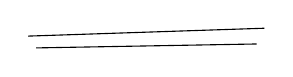
\begin{tikzpicture}\draw(0,0)--(3,.1);\draw(.1,-.15)--(2.9,-.1);\end{tikzpicture}}
Sous les \unsure{réserves|conditions} habituelles, \uline{si} $g:X/T\longrightarrow Y/T$ \uline{est de type fini}, \uline{alors} $f_*(g)$ \uline{est de type fini}.
[$S$ est \uline{loc. noeth.})
On est ramené au cas où $Y=T$, \deleted{$X$ affine} \inserted{Par} \deleted{sur $T$. On peut donc supposer} hypothèse, \deleted{\unsure{toute}} multisection d'un $X_s$ sur un $T_s$ est contenue dans un ouvert \deleted{\unsure{aff.}} \inserted{affine $U$}.
\unsure{Prouvons|Prenons} qu'un nb fini de tels ouverts affines \deleted{\unsure{X}} suffisent. \deleted{On peut supposer} \inserted{Soit en effet} \deleted{$S$ affine, dans le cas}
\[
\unsure{X^\nu}=\underbrace{X\times_S\unsure{-|\cdots}\times_S X}_{\nu},
\]
pour tt ouvert affine $U$ de $X$, soit
\[
U^\nu=\underbrace{U\times_S\unsure{-|\cdots}\times_S U}_{\nu},
\]
$U^\nu$ est un ouvert de $X^\nu$. \deleted{\unsure{Pour voir}} \inserted{Comme} $X^\nu$ est \deleted{\unsure{quasi}} noethérien, il existe un nb \uline{fini} d'ouverts affines $U_i$ tels que
\[
\bigcup U_i^\nu=\bigcup U^\nu.
\]
Soient $(x_1,-,x_\nu)\deleted{\in\unsure{(X_s)^\nu}\ \unsure{pris dans un même ouvert affine}}$ \deleted{$U$. Alors} soit $x\in X^\nu$ de projections les $x_i$. Alors les $x_i$ sont dans un ouvert affine
\margin{\uuline{\unsure{rédiger convenablement}}}
